\documentclass[crop,tikz]{standalone}
\usetikzlibrary{backgrounds}
\colorlet{blue}{cyan}
\tikzset{
  inverted/.style = {
    every path/.style = {draw=white,text=white},
    background rectangle/.style={fill},
    show background rectangle
  }
}

\tikzset{>=latex}
\usetikzlibrary{calc,decorations.markings,shapes}
\colorlet{gray}{gray!60}
\colorlet{green}{green}

\begin{document}
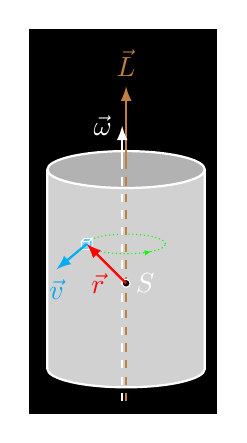
\begin{tikzpicture}[inverted,inverted]
  % cylinder
  \node (Z) at (0,0) [thick, cylinder, aspect=2, shape border rotate=90, draw, minimum height=3cm, minimum width=2cm, cylinder body fill=gray!60, cylinder uses custom fill, cylinder end fill=gray] {};
  % circular curve
  \draw[densely dotted,
        green,
        decoration={markings, mark=at position 0.9 with {\pgftransformscale{0.6}\arrow{>}}},
        postaction={decorate},
        ] (0,0.5) ellipse (0.5 and 0.125);
  % L
  \draw[dashed,brown,thick] (0,-1.5) -- +(0,3);
  \draw[->,brown,thick] (0,1.5) -- +(0,1) node[above] {$\vec{L}$};
  % omega
  \draw[dashed,thick] (-0.05,-1.5) -- +(0,3);
  \draw[->,thick] (-0.05,1.5) -- +(0,0.5) node[left] {$\vec{\omega}$};
  % center of mass
  \coordinate (CMS) at (0,0);
  \draw[fill] (CMS) circle (0.05) node[right] {$S$};
  % little piece of mass
  \coordinate (R) at ($(CMS)+(-0.5,0.5)$);
  % cube
  \pgfmathsetmacro{\cubex}{0.1}
  \pgfmathsetmacro{\cubey}{0.1}
  \pgfmathsetmacro{\cubez}{0.1}
  \coordinate (C) at ($(R)+(\cubex/2,\cubey/2,\cubez/2)$);
  \draw[fill=blue!50] (C) -- ++(-\cubex,0,0) -- ++(0,-\cubey,0) -- ++(\cubex,0,0) -- cycle;
  \draw[fill=blue!70] (C) -- ++(0,0,-\cubez) -- ++(0,-\cubey,0) -- ++(0,0,\cubez) -- cycle
                      (C) -- ++(-\cubex,0,0) -- ++(0,0,-\cubez) -- ++(\cubex,0,0) -- cycle;
  % arrows
  \draw[->,red,thick] (CMS) -- node[below,xshift=-0.3em] {$\vec{r}$} (R);
  \draw[->,blue,thick] (R) -- +(220:0.5) node[below] {$\vec{v}$};
\end{tikzpicture}
\end{document}
